\documentclass{ctexart}

\usepackage{graphicx}
\usepackage{amsmath}
\usepackage{amsfonts,amssymb}
\usepackage{algorithm}
\usepackage{algpseudocode}
\usepackage[export]{adjustbox}
\usepackage{subcaption}
\usepackage{tikz}

\usetikzlibrary{shapes,arrows,positioning}

\begin{document}
\pagestyle{empty}

\title{期末作业\\利用GSL求解方程$f(x)=0$的探索}
\author{张立言\\数学与应用数学\\3210101207}
\maketitle

\begin{abstract}
GSL是一个十分强大的科学计算库。利用其提供的求解方程根的函数,快速求解出一般方程的根。本文主要探讨二分法、牛顿法以及其他迭代方法求解不同方程的数学原理,并且利用计算机实现出来,比较和分析了不同迭代方法的收敛性和收敛速度。
\end{abstract}
\section{数学理论}
利用迭代方法,使得计算机能够求解方程的数值解。下面我们讨论两种最简单的迭代求解方法。

二分法适用于连续函数是一种方程式根的近似值求法。它是基于连续函数的介值性质以及实数的闭区间套定理推导出来。

牛顿迭代(Newton's method)又称为牛顿-拉佛森方法(Newton-Raphson method),它是一种在y实数域和复数域上近似求解方程的方法。方法使用函数$f(x)$的泰勒级数的前面几项来寻找方程$f(x)=0$的根。

\section{算法}
两种迭代方法的实现都不困难。我们可以了解它们的算法实现。这对于我们理解收敛性很有帮助。
\subsection{二分法 Bisection}
二分法的思路十分简单,它要求我们求解的$f(x)=0$中的$f(x)$为连续函数。算法流程如下:

\tikzstyle{decision} = [diamond, draw, fill=blue!20, aspect=2,
    text width=5em, text badly centered, node distance=3cm, inner sep=0pt]
\tikzstyle{block} = [rectangle, draw, fill=blue!20, 
    text width=5em, text centered, rounded corners, minimum height=4em]
\tikzstyle{line} = [draw, -latex']
\tikzstyle{cloud} = [draw, ellipse,fill=red!20, node distance=3cm,text width=7em,
    minimum height=2em]
\begin{figure}[H]    
\begin{tikzpicture}[node distance = 4cm, auto]
  \node[cloud] (require) {Given $f(x)$ and interval $[a,b]$, $f(a)f(b)<0$};
  \node [decision, below of=require] (0) {$f(\frac{a+b}{2})=0$ or $|a-b|<\varepsilon$?};
  \node [block, below of=0] (give) {$a=\frac{a+b}{2}$};
  \node [decision,left of=give, text width=7em] (a) {$f(a)f(\frac{a+b}{2})>0$};
  \node [decision,right of=give,text width=7em] (b) {$f(a)f(\frac{a+b}{2})>0$};
  \node [block, below of=a] (aa) {$a=\frac{a+b}{2}$};
  \node [block, below of=b] (bb) {$b=\frac{a+b}{2}$};
  \node [draw, rounded rectangle, fill=green!20, text width=10em,text centered,minimum height=5em,  below=8cm of 0] (solve) {Root = $\frac{a+b}{2}$};
  \path [line] (require) -- (0);
  \path [line] (0) -| (a);
  \path [line] (0) -| (b);
  \path [line] (0) -- (give);
  \path [line] (a) -- (aa);
  \path [line] (b) -- (bb);
  \path [line] (give) -- (solve);
  \draw [black] (aa) -- (-5,-11);
  \draw [black] (-5,-11) -- (-5,-2);
  \path [line] (-5,-2) -- (0);
  \draw [black] (bb) -- (5,-11);
  \draw [black] (5,-11) -- (5,-2);
  \path [line] (5,-2) -- (0);
\end{tikzpicture}
\end{figure}
\subsection{牛顿法 Newton's method}
其算法的实现更加简单,只要正确规定迭代停止的条件即可。

\section{数值算例}
\subsection{不同的迭代方法}
我们首先以求解方程$f(x)=x^2-5=0$为例,让程序同时运行二分法和牛顿迭代法,判断其收敛性。我们设置最大迭代次数为100,迭代停止条件是间隔小于0.001:

\begin{figure}[H]
  \centering
  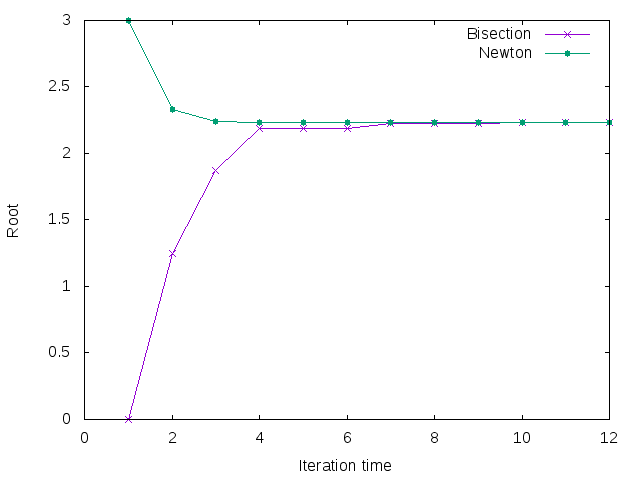
\includegraphics[width=0.7\textwidth]{graph1.png}
  \caption{Solving $x^2-5=0$ using bisection and newton method}
\end{figure}

从图中我们可以看到,二分法以下界作为根的近似值。求解方程的迭代次数都没有超过最大迭代次数100,而牛顿迭代法只需要4次即可达到迭代停止条件。

同样的,GSL也提供了其他的迭代方法。以不需要导数的迭代为例,我们可以采用布伦特方法(Brent's method),在GSL中可以调用相关函数即可。我们进行同样的操作,与牛顿迭代法进行比较,得到如下图像:

\begin{figure}[H]
  \centering
  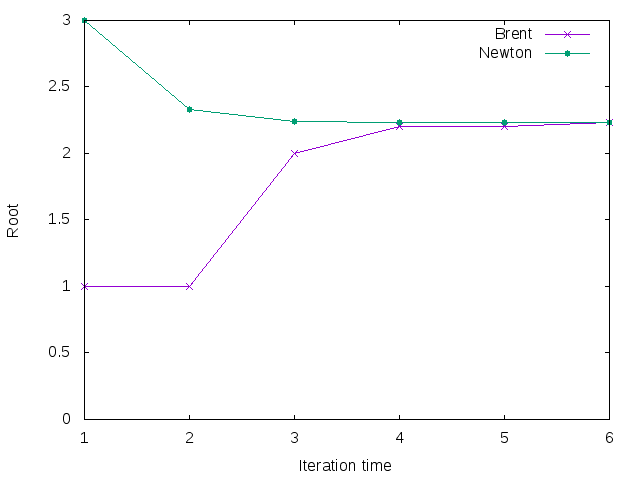
\includegraphics[width=0.7\textwidth]{graph2.png}
  \caption{Solving $x^2-5=0$ using brent and newton method}
\end{figure}

Brent比起二分法,迭代次数大大减少,只需要迭代6次就能够达到停止条件。但是从输出的数据文件来看,牛顿法迭代次数仍然少于Brent方法。比起不需要导数的迭代,牛顿法有着更明显的优势。

仍然以方程$x^2-5=0$为例,我们再比较一下Newton method和斜截法(Secant)。整理运行的数据得到如下示意图:

\begin{figure}[H]
  \centering
  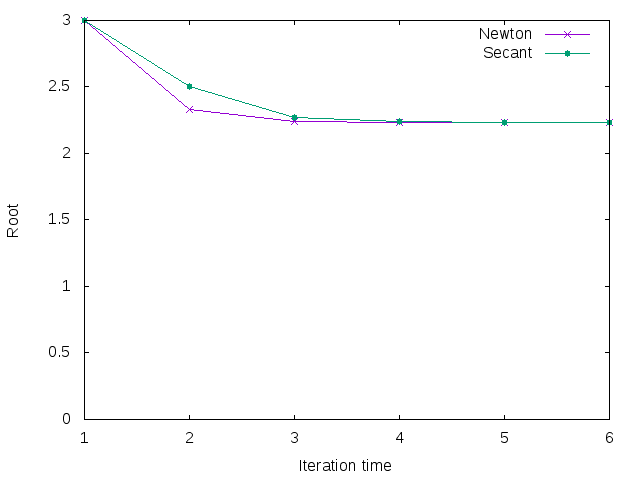
\includegraphics[width=0.7\textwidth]{graph3.png}
  \caption{Using Newton method and secant method}
\end{figure}

从图中我们可以看到,虽然它们都是在迭代6次后就达到停止条件,但是牛顿法的收敛速度明显快于斜截法。这与我们直观的想法是一致的,因为斜截法的表达式中"导数"是离散化的。

\subsection{解一下超越方程}
我们使用二分法和牛顿法解一个简单的超越方程:$f(x)=e^x-4x=0$.我们首先看一下它在$[0,3]$的大致图像:

\begin{figure}[H]
  \centering
  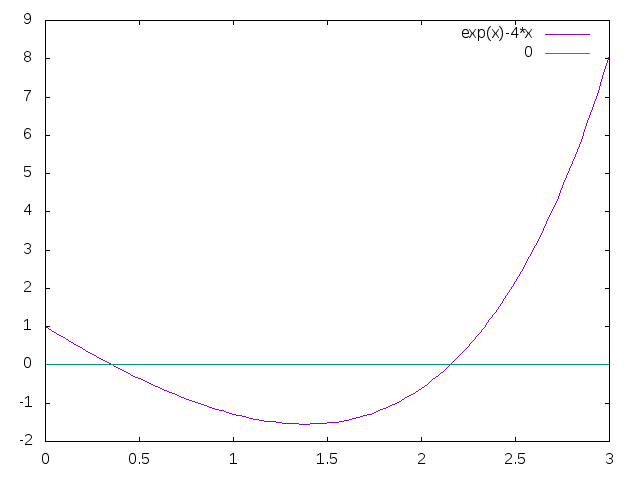
\includegraphics[width=0.7\textwidth]{f.png}
  \caption{Image of $f(x)$}
\end{figure}

由此我们确定根的区间为$[0,3]$,观察最终解的位置。
\begin{figure}[H]
  \begin{subfigure}{0.7\linewidth}
  \centering
  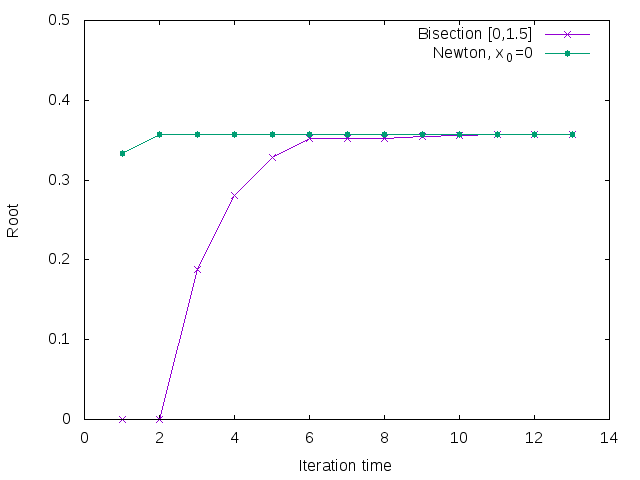
\includegraphics[width=0.5\textwidth]{graph4.png}
  \end{subfigure}
  \begin{subfigure}{0.7\linewidth}
  \centering
  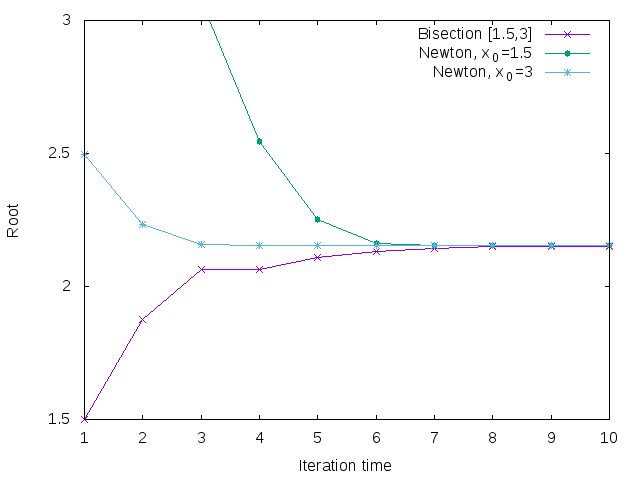
\includegraphics[width=0.5\textwidth]{graph5.png}
  \end{subfigure}
  \caption{Different initial values, and bisection}
\end{figure}

首先让牛顿迭代的初值分别为0,1.5和3,最终都收敛到了较大的根,由图中可以观察到,选取初值$x_0=3$的时候,收敛的速度跟快。二分法由于区间的限制,必定收敛于某一个大根或者小根,相比于两次牛顿迭代,二分法仍然没有优势。

\section{分析}
有关二分法和牛顿法的收敛效果,我们可以由如下的一些定理进行描述:

\textbf{Theorem 1}{} 二分法达到精度$\varepsilon$,需要的最大迭代次数$N$满足:
\begin{equation}
  N \ge \frac{ln(b_0-a_0)-ln(\varepsilon)}{ln(2)}
\end{equation}

因为$varepsilon$在对数下,当$\varepsilon$很小的时候,需要的迭代次数会急剧增大。

\textbf{Theorem 2}{} 对于牛顿迭代法,有:
\begin{equation}
   \lim_{k \to \infty} \frac{e_{k+1}}{e_k^2} = |f''(\xi)|
\end{equation}
在这里,$e_k$表示第k次迭代的误差。\par
由上面的定理我们可以发现,牛顿迭代法的误差会以指数上的指数的级别缩小。所以说牛顿迭代法具有更好的收敛效果。\par
\textbf{Theorem 3}{} 对于斜截法,有:
\begin{equation}
   \lim_{k \to \infty} \frac{e_{k+1}}{e_k^{\alpha}} = |f''(\xi)|
   where \alpha=\frac{1+\sqrt{5}}{2}
\end{equation}
通过简单的计算,我们知道$\alpha < 2$,这一点说明了斜截法相对于牛顿迭代,收敛效果较差。但是斜截法也有优点,它适用于于导数难以计算或者导数未知的方程求解,但是牛顿法对此无能为力。\par
这些理论与我们实验中的数据的直观性质一致。
\section{总结}
这次实验充分利用了GSL来进行科学计算,同时也让我们看到了不同的算法求解同一个问题,虽然理论上的最终结果都是相同的,但是由于计算机只能处理离散的数据,我们要尽可能的通过离散的数据处理去接近精确的数学理论,这就体现出了不同算法的相对优势。
\end{document}
